%% Creator: Inkscape inkscape 0.91, www.inkscape.org
%% PDF/EPS/PS + LaTeX output extension by Johan Engelen, 2010
%% Accompanies image file 'setup.pdf_tex.pdf' (pdf, eps, ps)
%%
%% To include the image in your LaTeX document, write
%%   \input{<filename>.pdf_tex}
%%  instead of
%%   \includegraphics{<filename>.pdf}
%% To scale the image, write
%%   \def\svgwidth{<desired width>}
%%   \input{<filename>.pdf_tex}
%%  instead of
%%   \includegraphics[width=<desired width>]{<filename>.pdf}
%%
%% Images with a different path to the parent latex file can
%% be accessed with the `import' package (which may need to be
%% installed) using
%%   \usepackage{import}
%% in the preamble, and then including the image with
%%   \import{<path to file>}{<filename>.pdf_tex}
%% Alternatively, one can specify
%%   \graphicspath{{<path to file>/}}
%% 
%% For more information, please see info/svg-inkscape on CTAN:
%%   http://tug.ctan.org/tex-archive/info/svg-inkscape
%%
\begingroup%
  \makeatletter%
  \providecommand\color[2][]{%
    \errmessage{(Inkscape) Color is used for the text in Inkscape, but the package 'color.sty' is not loaded}%
    \renewcommand\color[2][]{}%
  }%
  \providecommand\transparent[1]{%
    \errmessage{(Inkscape) Transparency is used (non-zero) for the text in Inkscape, but the package 'transparent.sty' is not loaded}%
    \renewcommand\transparent[1]{}%
  }%
  \providecommand\rotatebox[2]{#2}%
  \ifx\svgwidth\undefined%
    \setlength{\unitlength}{1567.76523438bp}%
    \ifx\svgscale\undefined%
      \relax%
    \else%
      \setlength{\unitlength}{\unitlength * \real{\svgscale}}%
    \fi%
  \else%
    \setlength{\unitlength}{\svgwidth}%
  \fi%
  \global\let\svgwidth\undefined%
  \global\let\svgscale\undefined%
  \makeatother%
  \begin{picture}(1,0.56250002)%
    \put(0,0){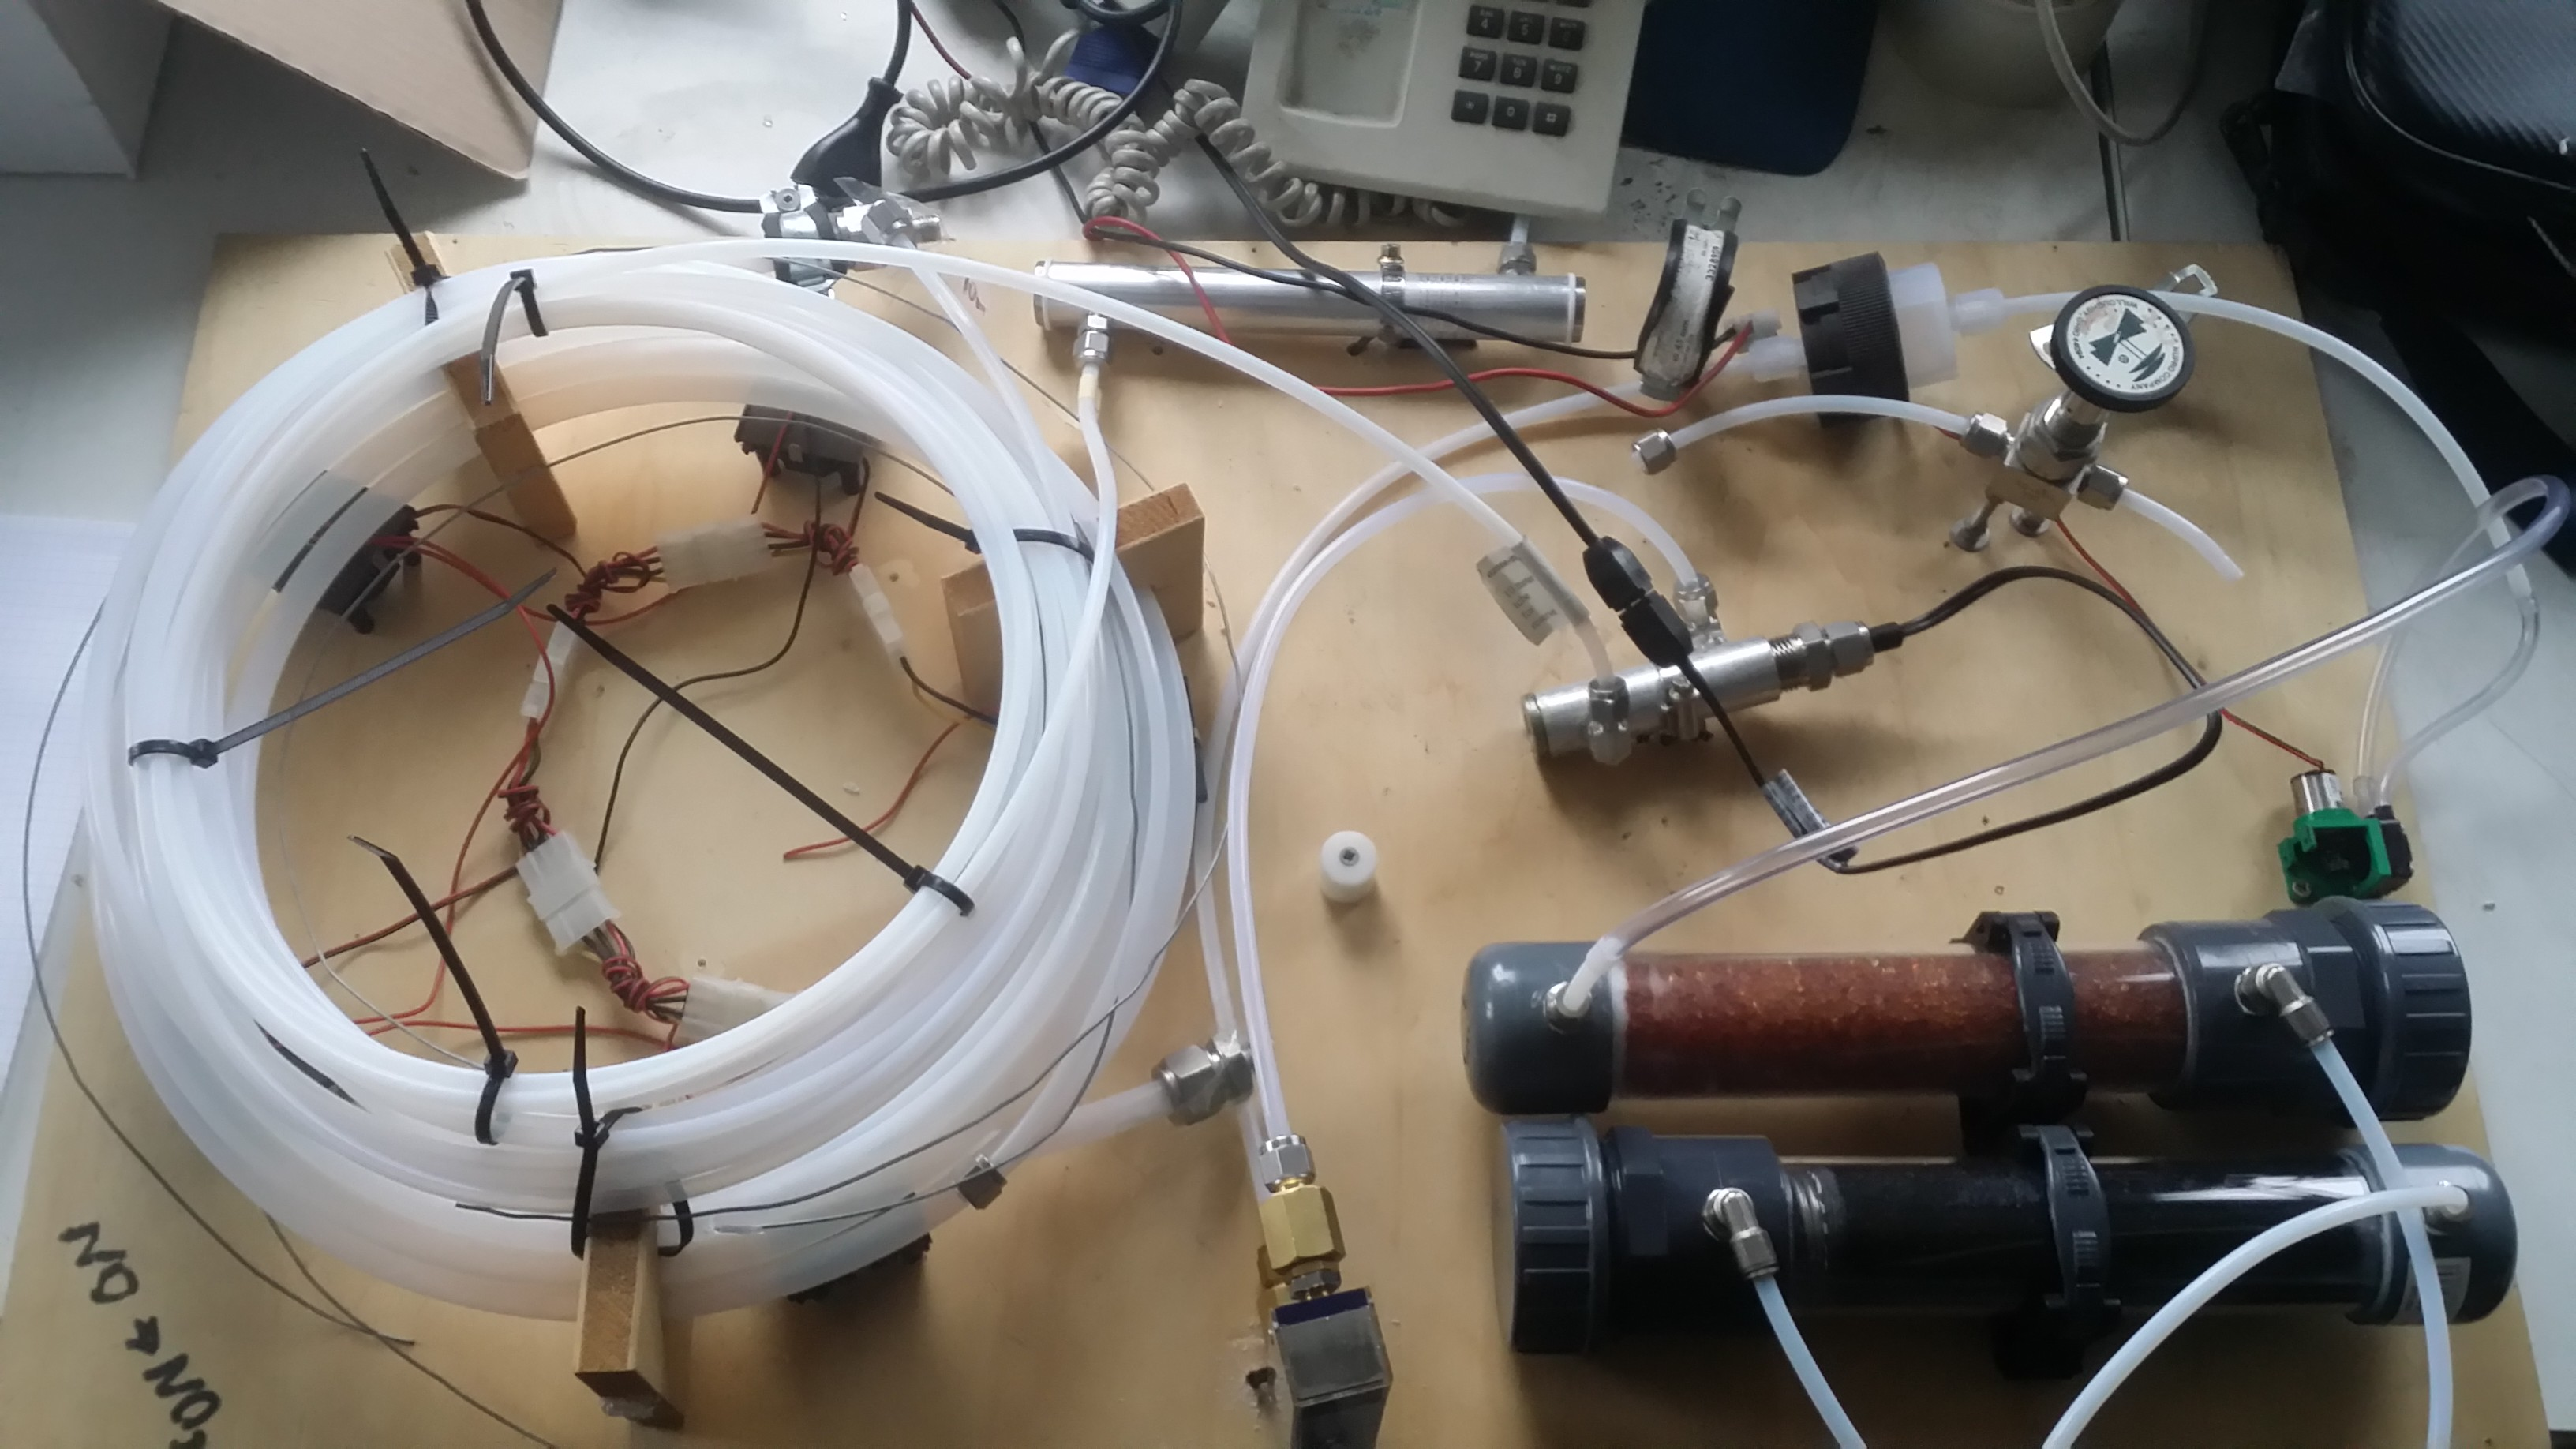
\includegraphics[width=\unitlength,page=1]{setup.pdf}}%
    \put(0.72339254,0.0272422){\color[rgb]{0,0,0}\makebox(0,0)[lb]{carbon filter}}%
    \put(0.68467052,0.20608212){\color[rgb]{0,0,0}\makebox(0,0)[lb]{\smash{silica gel}}}%
    \put(0.84485225,0.27636329){\color[rgb]{0,0,0}\makebox(0,0)[lb]{\smash{pump}}}%
    \put(0.66524548,0.47215208){\color[rgb]{0,0,0}\makebox(0,0)[lb]{\smash{particle filter}}}%
    \put(0.37854499,0.02340413){\color[rgb]{0,0,0}\makebox(0,0)[lb]{\smash{flowmeter}}}%
    \put(0.41093385,0.46876799){\color[rgb]{0,0,0}\makebox(0,0)[lb]{\smash{silica gel in tube}}}%
    \put(0.55474278,0.26558162){\color[rgb]{0,0,0}\makebox(0,0)[lb]{\smash{penray lamp in tube}}}%
    \put(0,0){\includegraphics[width=\unitlength,page=2]{setup.pdf}}%
    \put(1.00286136,0.04729665){\color[rgb]{0,0,0}\makebox(0,0)[lb]{\smash{lab air}}}%
    \put(0.59985726,0.5399915){\color[rgb]{0,0,0}\makebox(0,0)[lb]{\smash{ozone}}}%
    \put(0,0){\includegraphics[width=\unitlength,page=3]{setup.pdf}}%
  \end{picture}%
\endgroup%

%%% Local Variables:
%%% mode: latex
%%% TeX-master: "../Bachelor"
%%% End:
